%%%%%%%%%%%%%%%%%%%%%%%%%%%%%%%%%%%%%%%%%
% Document Author: Plinio H. Vargas
% Course: CS-532, Spring 2016 at Old Dominion University
%
% Structured General Purpose Assignment
% LaTeX Template
%
% This template has been downloaded from:
% http://www.latextemplates.com
%
% Original template author:
% Ted Pavlic (http://www.tedpavlic.com)
%
% Note:
% The \lipsum[#] commands throughout this template generate dummy text
% to fill the template out. These commands should all be removed when 
% writing assignment content.
%
%%%%%%%%%%%%%%%%%%%%%%%%%%%%%%%%%%%%%%%%%
%----------------------------------------------------------------------------------------
%	PACKAGES AND OTHER DOCUMENT CONFIGURATIONS
%----------------------------------------------------------------------------------------

\documentclass{article}

\usepackage{fancyhdr} % Required for custom headers
\usepackage{lastpage} % Required to determine the last page for the footer
\usepackage{extramarks} % Required for headers and footers
\usepackage{listings}
\usepackage{graphicx} % Required to insert images
\usepackage{lipsum} % Used for inserting dummy 'Lorem ipsum' text into the template
\usepackage[bookmarks,bookmarksopen,bookmarksdepth=2]{hyperref} % for bookmarks
\usepackage{enumerate}
\usepackage{csquotes} % for quoting things
\usepackage{multirow}
\usepackage{amsmath}
\usepackage{navigator}
\usepackage{caption}
\usepackage[shortlabels]{enumitem}
\usepackage{lmodern}
\usepackage[utf8]{inputenc}
%\usepackage[table]{xcolor}% http://ctan.org/pkg/xcolo
\usepackage[dvipsnames]{xcolor}
\usepackage{longtable}
\usepackage{textcomp}
\usepackage{url}
\usepackage{import}
\usepackage{float}
\usepackage{dashrule} % for dashline
\usepackage{keystroke}

\lstdefinestyle{numbers}
{ frame=tb,
  language=python,
  aboveskip=3mm,
  belowskip=3mm,
  showstringspaces=false,
  columns=flexible,
  basicstyle={\small\ttfamily},
  numbers=left,
  numberstyle=\tiny\color{gray},
  keywordstyle=\color{blue},
  commentstyle=\color{OliveGreen},
  stringstyle=\color{purple},
  breaklines=true,
  breakatwhitespace=true,
  tabsize=3
}

\lstdefinestyle{nonumbers}
{ frame=shadowbox,
  language=python,
  aboveskip=3mm,
  belowskip=3mm,
  showstringspaces=false,
  columns=flexible,
  basicstyle={\small\ttfamily},
  numbers=none,
  numberstyle=\tiny\color{gray},
  keywordstyle=\color{blue},
  commentstyle=\color{OliveGreen},
  stringstyle=\color{purple},
  breaklines=true,
  breakatwhitespace=true,
  tabsize=3
}
% Margins
\topmargin=-0.45in
\evensidemargin=0in
\oddsidemargin=0in
\textwidth=6.5in
\textheight=9.0in
\headsep=0.25in 

\linespread{1.1} % Line spacing
\newcommand*{\meda}{\mathbin{\scalebox{1.5}{a}}}% increase size of letter a
\newcommand\multibrace[3]{\rdelim\}{#1}{3mm}[\pbox{#2}{#3}]}

% Set up the header and footer
\pagestyle{fancy}
\lhead{\hmwkAuthorName} % Top left header
\chead{\hmwkShortClass\ (\hmwkClassInstructor\ \hmwkClassTime): \hmwkShortTitle} % Top center header
%\rhead{\firstxmark} % Top right header
\rhead{} % Top right header
\lfoot{\lastxmark} % Bottom left footer
\cfoot{} % Bottom center footer
\rfoot{Page\ \thepage\ of\ \pageref{LastPage}} % Bottom right footer
\renewcommand\headrulewidth{0.4pt} % Size of the header rule
\renewcommand\footrulewidth{0.4pt} % Size of the footer rule

\setlength\parindent{0pt} % Removes all indentation from paragraphs

%----------------------------------------------------------------------------------------
%	DOCUMENT STRUCTURE COMMANDS
%	Skip this unless you know what you're doing
%----------------------------------------------------------------------------------------

% Header and footer for when a page split occurs within a problem environment
\newcommand{\enterProblemHeader}[1]{
\nobreak\extramarks{#1}{#1 continued on next page\ldots}\nobreak
\nobreak\extramarks{#1 (continued)}{#1 continued on next page\ldots}\nobreak
}

% Header and footer for when a page split occurs between problem environments
\newcommand{\exitProblemHeader}[1]{
\nobreak\extramarks{#1 (continued)}{#1 continued on next page\ldots}\nobreak
\nobreak\extramarks{#1}{}\nobreak
}

\setcounter{secnumdepth}{0} % Removes default section numbers
\newcounter{homeworkProblemCounter} % Creates a counter to keep track of the number of problems

\newcommand{\homeworkProblemName}{}
\newenvironment{homeworkProblem}[1][Problem \arabic{homeworkProblemCounter}]{ % Makes a new environment called homeworkProblem which takes 1 argument (custom name) but the default is "Problem #"
\stepcounter{homeworkProblemCounter} % Increase counter for number of problems
\renewcommand{\homeworkProblemName}{#1} % Assign \homeworkProblemName the name of the problem
\section{\homeworkProblemName} % Make a section in the document with the custom problem count
\enterProblemHeader{\homeworkProblemName} % Header and footer within the environment
}{
\exitProblemHeader{\homeworkProblemName} % Header and footer after the environment
}

\newcommand{\problemAnswer}[1]{ % Defines the problem answer command with the content as the only argument
\noindent\framebox[\columnwidth][c]{\begin{minipage}{0.98\columnwidth}#1\end{minipage}} % Makes the box around the problem answer and puts the content inside
}

\newcommand{\homeworkSectionName}{}
\newenvironment{homeworkSection}[1]{ % New environment for sections within homework problems, takes 1 argument - the name of the section
\renewcommand{\homeworkSectionName}{#1} % Assign \homeworkSectionName to the name of the section from the environment argument
\subsection{\homeworkSectionName} % Make a subsection with the custom name of the subsection
\enterProblemHeader{\homeworkProblemName\ [\homeworkSectionName]} % Header and footer within the environment
}{
\enterProblemHeader{\homeworkProblemName} % Header and footer after the environment
}
   
%----------------------------------------------------------------------------------------
%	NAME AND CLASS SECTION
%----------------------------------------------------------------------------------------

\newcommand{\hmwkTitle}{\\Assignment\ \#2} % Assignment title
\newcommand{\hmwkShortTitle}{Assignment 2} % Assignment title
\newcommand{\hmwkDueDate}{Thursday,\ February 11,\ 2016} % Due date
\newcommand{\hmwkClass}{CS-432/532 Introduction to Web Science} % Course/class
\newcommand{\hmwkShortClass}{CS-432/532 Web Science} % Course/class
\newcommand{\hmwkClassTime}{- Spring 2016} % Class/lecture time
\newcommand{\hmwkClassInstructor}{Dr.  Michael L. Nelson} % Teacher/lecturer
\newcommand{\hmwkAuthorName}{Plinio Vargas} % Your name
\newcommand{\hmwkAuthorEmail}{pvargas@cs.odu.edu} % Your name
%------------------------------------------------------------
% Algorithm declaration
%------------------------------------------------------------
\lstnewenvironment{algorithm}[1][] %defines the algorithm listing environment
{   
    %\refstepcounter{nalg} %increments algorithm number
    \captionsetup{labelsep=colon} %defines the caption setup for: it ises label format as the declared caption label above and makes label and caption text to be separated by a ':'
    \lstset{ %this is the stype
        frame=tB,
        numbers=left, 
        mathescape=true,
        numberstyle=\tiny,
        basicstyle={\small\ttfamily}, 
        keywordstyle=\color{blue}\bfseries\em,
        keywords={,input, output, return, 
                   datatype, function, in, 
                   if, else, for, foreach, 
                   while, write, begin, end, 
        } %add the keywords you want, or load a language as Rubens explains in his comment above.
        numbers=left,
        xleftmargin=.04\textwidth,
        #1 % this is to add specific settings to an usage of this environment (for instnce, the caption and referable label)
    }
}
{}
%----------------------------------------------------------------------------------------
%	TITLE PAGE
%----------------------------------------------------------------------------------------

\title{
\vspace{2in}
\textmd{\textbf{\hmwkClass:\ \hmwkTitle}}\\
\normalsize\vspace{0.1in}\small{Due\ on\ \hmwkDueDate}\\
\vspace{0.1in}\large{\textit{\hmwkClassInstructor\ }}
\vspace{3in}
}

\author{\textbf{\hmwkAuthorName} \\ \hmwkAuthorEmail}
\date{} % Insert date here if you want it to appear below your name

%----------------------------------------------------------------------------------------
%	EMBEDDED FILE
%----------------------------------------------------------------------------------------
\embeddedfile{TwitterURI.py}{../TwitterURI.py}
\embeddedfile{Links}{../linkfiles.txt}
\embeddedfile{Mementos}{../MementosURI.py}
\embeddedfile{Histogram}{../histogram.r}
\embeddedfile{URIage}{../AgeURI.py}
\embeddedfile{AgeMemntoPlot}{../ageplot.R}
\embeddedfile{AgeMementoPlotSize}{../ageplotsize.R}
%----------------------------------------------------------------------------------------
%	START OF DOCUMENT
%----------------------------------------------------------------------------------------
\begin{document}

\clearpage\maketitle
\thispagestyle{empty}

%----------------------------------------------------------------------------------------
%	TABLE OF CONTENTS
%----------------------------------------------------------------------------------------

%\setcounter{tocdepth}{1} % Uncomment this line if you don't want subsections listed in the ToC

\newpage
\clearpage\tableofcontents
\listoffigures
\listoftables

\thispagestyle{empty}
\newpage
\setcounter{page}{1}
%----------------------------------------------------------------------------------------
%	Prefaces
%----------------------------------------------------------------------------------------
\section{Preface} % Custom section title
\vspace*{10pt} % Question
Since the course material will become more complex as the semester progresses, and knowing that many solutions to new problems can be built on previous ones, I decided to create a library to access and re-utilize code.\\

Some of these functions can be really small (4-7 lines), however they solve a specific problem, so it is better to separate them from the rest of the code.\\

The location, interaction and functionality of this library, and the directory structure for this assignment are presented in more detail in the README file within the same folder hierarchy where this file was found.

%----------------------------------------------------------------------------------------
%	Problem 1
%----------------------------------------------------------------------------------------
\begin{homeworkProblem} % Custom section title
\vspace*{10pt} % Question
Write a Python program that extracts 1000 unique links from
Twitter.  You might want to take a look at:\\

url{http://thomassileo.com/blog/2013/01/25/using-twitter-rest-api-v1-dot-1-with-python/}\\

But there are many other similar resources available on the web.  Note
that only Twitter API 1.1 is currently available; version 1 code will
no longer work.\\

Also note that you need to verify that the final target URI (i.e., the
one that responds with a 200) is unique.  You could have many different
shortened URIs for www.cnn.com (t.co, bit.ly, goo.gl, etc.).\\
\vspace{10mm}

\subsection{1.1 Approach}
\begin{figure}[!h]
\caption{Flowchart diagram for \textit{TwitterURI.py}}\label{fig:0}
\center
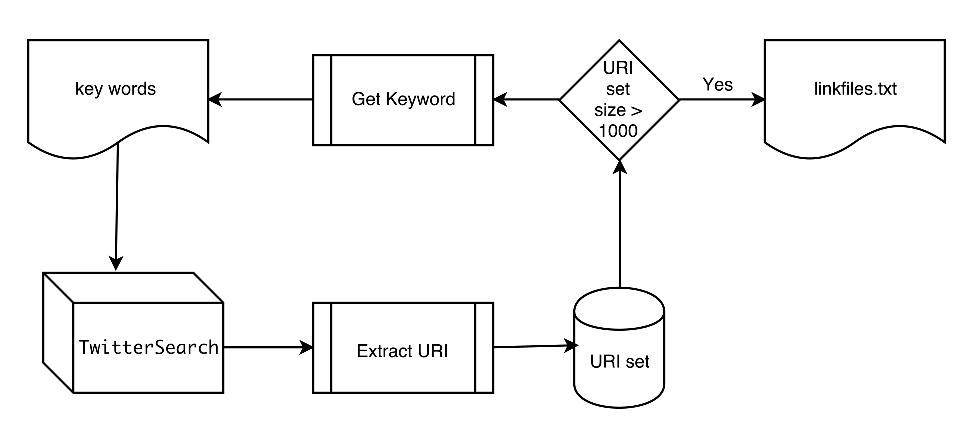
\includegraphics[scale=.5]{images/createlinks.pdf}
\caption*{\scriptsize \textit{\textbf{TwitterURI.py}} is the Python program solution for problem 1. \textbf{keywords} is a text file document which contains subject of interest, such as baseball, \enquote{Dominican, Republic}, etc.; \textbf{TwitterSeach} is an API that provides a set of tweets from Twitter given a particular keyword; \textbf{Extract URI} filters any URI within the tweet; \textbf{URI set} is a unique collection of URIs; \textbf{Get Keyword} gets the next keyword from the text file; and finally \textbf{\textit{linkfiles.txt}} is a collection of 1000 unique URIs.}
\end{figure}
Since we do not know the number of tweets returned from a particular keyword search,  a file was created (\textit{keywords.txt}) as input for \textit{\textbf{TwitterURI.py}} (lines 70-75). Then, the API \textbf{TwitterSeach} in line (28-34) is used, which returns $n$ number of tweets. From the tweet object we can extract the URI using regular expression (line 44):\\
\begin{lstlisting}[style=nonumbers]
            url = re.findall(r'(https?://[^\s]+)', tweet['text'])
\end{lstlisting}
The extracted URI is validated and placed in a set: \textit{all\_links\_set} lines (49-54):
\begin{lstlisting}[style=nonumbers]
                # check if url has been already used
                if uri not in root_url_array:
                    root_url_array.append(uri)

                    if validators.url(uri):
                        AddURI(all_links_set, uri)
\end{lstlisting}
The last line of the portion code above uses a function \textit{AddURI} imported from the self developed library \textit{WEBlib.py} (a collection of functions that may have use for future applications). The function takes as a parameter a set object and a string (uri). \textit{AddURI} takes care of all details regarding request response, connection timeouts, resource redirects, etc. ONLY if final URI provides a response 200 it gets added to the set.\\

Finally, if the set size is not greater than or not equal to 1000, we continue to get more keywords and repeat the process, otherwise the deliverable (1000 unique URIs) is written in \textit{linkfiles.txt}.
\subsection{1.2 Solution}
See attached embedded file: \textbf{\textit{linkfiles.txt}}\\
Below is the entire code \textit{\textbf{TwitterURI.py}}, which is also attached to this document.
\import{./}{TwitterURI.tex}
\end{homeworkProblem}

%----------------------------------------------------------------------------------------
%	Problem 2
%----------------------------------------------------------------------------------------
\begin{homeworkProblem}
Download the TimeMaps for each of the target URIs.  We'll use the ODU 
Memento Aggregator, so for example: \\

URI-R = http://www.cs.odu.edu/\\

URI-T = http://mementoproxy.cs.odu.edu/aggr/timemap/link/1/http://www.cs.odu.edu/\\

Create a histogram* of URIs vs. number of Mementos (as computed from
the TimeMaps).  For example, 100 URIs with 0 Mementos, 300 URIs
with 1 Memento, 400 URIs with 2 Mementos, etc.\\

* = https://en.wikipedia.org/wiki/Histogram\\

\subsection{2.1 Approach}
A Python code $<\textbf{\textit{MementosURI.py}}>$ was developed to generate the histogram data, and the Histogram Graph (Figure \ref{fig:1}) was generated using R-code $<histogram.r>$. Both files are attached to this document. Since we will be using the data collected later on in the course, a folder \textbf{a2/mementodata} was created to hold all TimeMaps for URIs included in $<linkfiles.txt>$ (solution to problem 1).\\

URIs in $<linkfiles.txt>$ are written sequentially and only separated by a new-line character (`$\backslash$n'). In order to make a relation TimeMap-URI, the following file name format was established:
$$date\_created.relative\_position$$
For example if file \textit{20160204.21} is located in folder \textbf{a2/mementodata}, then it references the TimeMap for URI located in position 21 out of 1000 in file  $<linkfiles.txt>$. If \textit{20160204.1} is not found in the directory, then there is no TimeMap for the first URI in $<linkfiles.txt>$.\\

Given the schema to solve Problem 2, below is the pseudo-code used for its implementation:
\newpage
\begin{algorithm}[caption={MementosURI.py Pseudo Code},]
 input: (I) file linkfiles.txt 
 output: (O) file histogramdata
 Let A be an empty array where index $i$ is number of mementos.
 Let D be an stack containing all filenames in directory a2/mementodata
 Let S be an integer containing number of URIs in I
 
 # Initialize URIs with zero memento to number of URIs in I
 A[0] $\gets$ S
 
 begin
    while file in D
       A[0] $\gets$ A[0] - 1   # decrease number URIs with zero mementos
       $i \gets$ number of memento in file
       D.pop()
       if $i\ \in$ A then
          A[$i$] $\gets$ A[$i$] + 1      
       else
          A[$i$] $\gets$ 1
      
       for $k:=1\ \to$ A.size
          write into O ($k$, A[$k$])
 end       
\end{algorithm}
\vspace{5mm}
The python implementation found in $<\textbf{\textit{MementosURI.py}}>$ and pseudo-code above  are very similar, and straightforward if we remove all exception handling required for the implementation. The input file $I$ is used to get the number of URIs in our sample $S$ (1000). $O$ is the output file where histogram data will be saved. $D$ contains all file names that have TimeMaps. Array $A$ contains the data that will be written as a tuple in $O$. $A$ starts as an empty array, so ONLY the indexes with values will be saved. \\

Different from the pseudo-code will be using instead of an array $A$ a dictionary object \cite{Lutz} in the Python implementation.\\

Then, the only worthwhile explanation is how to find the value of index $i$ or the number of mementos in any particular file. This is performed by the function \textit{GetNumberMementos(filename)} located in our developed library \textit{WEBlib.py}:
\begin{lstlisting}[style=nonumbers]
def GetNumberMementos(filename):
    """
    :param filename: Name of file to count number of mementos
    :return: number of mementos
    """
    with open(filename, 'r') as file:
        text = file.read()

    return len(re.findall(r'rel=\"memento\"', text))
\end{lstlisting}
\vspace{5mm}
As we may notice, function \textit{GetNumberMementos()} simple takes as an argument a file name. It opens the file for reading and it uses regular expression to count and return the number of rel=\enquote{memento} occurrences in the file.

\newpage
\subsection{2.2 Solution}
\begin{figure}[!h]
\caption{Memento Histogram for 1000 URIs Extracted from Twitter}\label{fig:1}
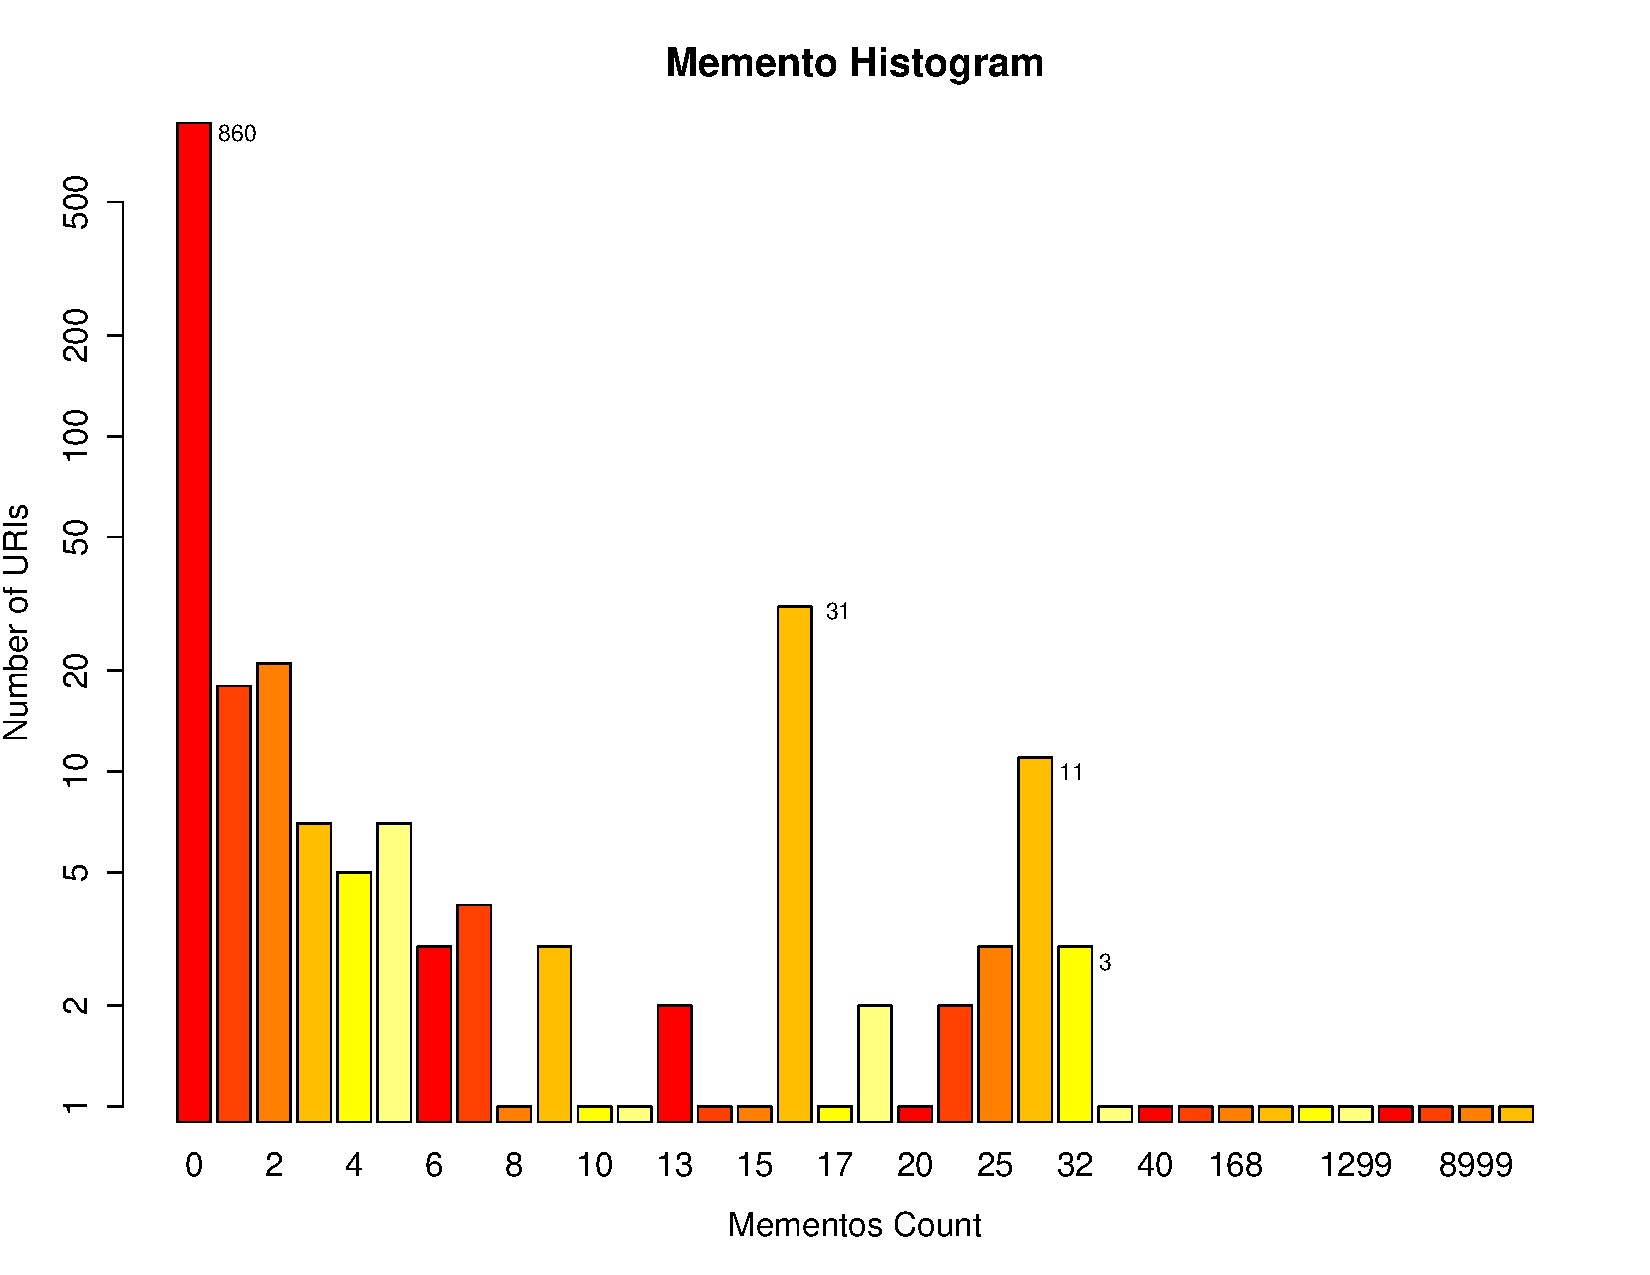
\includegraphics[scale=.5]{images/memHist.pdf}
\caption*{\scriptsize The y-axis or Number of URIs is in a log scale.  The data used to plot this histogram is contained in Table \ref{tab:table1}. The histogram resembles characteristics of a power-law distribution: (80/20) values. In our case 860 URIs out of a 1,000 had 0 mementos. At the tail end of the histogram we can notice that the memento counts gets higher as the number of URIs get smaller.}
\end{figure}

\end{homeworkProblem}
%----------------------------------------------------------------------------------------
%	Problem 3
%----------------------------------------------------------------------------------------
\newpage
\begin{homeworkProblem}
Estimate the age of each of the 1000 URIs using the "Carbon Date" tool:\\

http://ws-dl.blogspot.com/2014/11/2014-11-14-carbon-dating-web-version-20.html\\

Note: you'll should download the library and run it locally; don't
try to use the web service.\\

For URIs that have $> 0$ Mementos and an estimated creation date,
create a graph with age (in days) on one axis and number of mementos
on the other.  \\

Not all URIs will have Mementos, and not all URIs will have an estimated
creation date.  State how many fall into either categories.\\
\subsection{3.1 Approach}
We will be using the same nomenclature file schema to associate the Carbon Date data with an URI's age. However, the Carbon Date files will be stored in a different directory: \textbf{a2/uriagedata}. Similar to problem 2 approach, python was used to generate the data, and R was utilized to create the graphs.\\

Shown below is a flowchart diagram for a python program used to generate the data:

%
%                  AgeURI.py Flow Chart
%

\begin{figure}[!h]
\caption{Flowchart diagram for \textit{AgeURI.py}}\label{fig:3}
\center
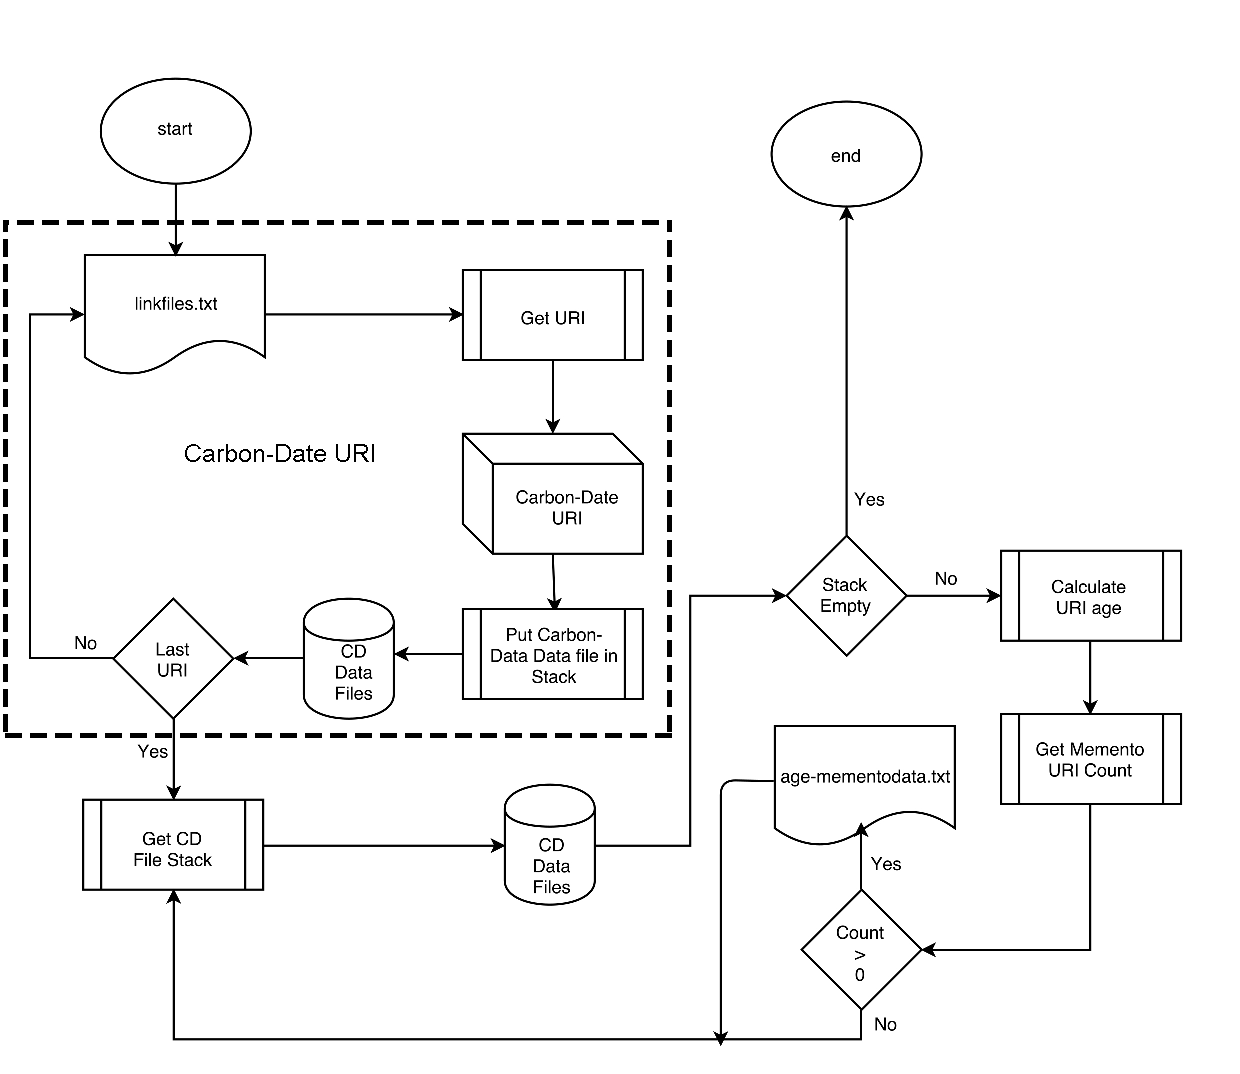
\includegraphics[scale=.5]{images/carbondate.pdf}
\caption*{\scriptsize \textit{\textbf{AgeURI.py}} is the Python implementation for problem 3. The section in the diagram labeled \textbf{Carbon-Date URI} takes all URIs generated to solve problem 1 and uses the \textbf{Carbon Date Tool} obtained from \url{http://ws-dl.blogspot.com/2014/11/2014-11-14-carbon-dating-web-version-20.html}. The HTTP request output is saved into \textbf{uriagedata} directory. This directory is labeled in the diagram \textbf{CD Data Files}. The remaining part of the flowchart explains that \textbf{CD Data Files} result gets merged with the result from data file solution from problem 2 (\textbf{Get Memento URI count} to produce our deliverable: \textbf{age-memento-data.txt} file.}
\end{figure}
%
\newpage
\subsection{3.2 Solution Part-1}
\begin{figure}[!h]
\caption{Age-Memento Graph}\label{fig:4}
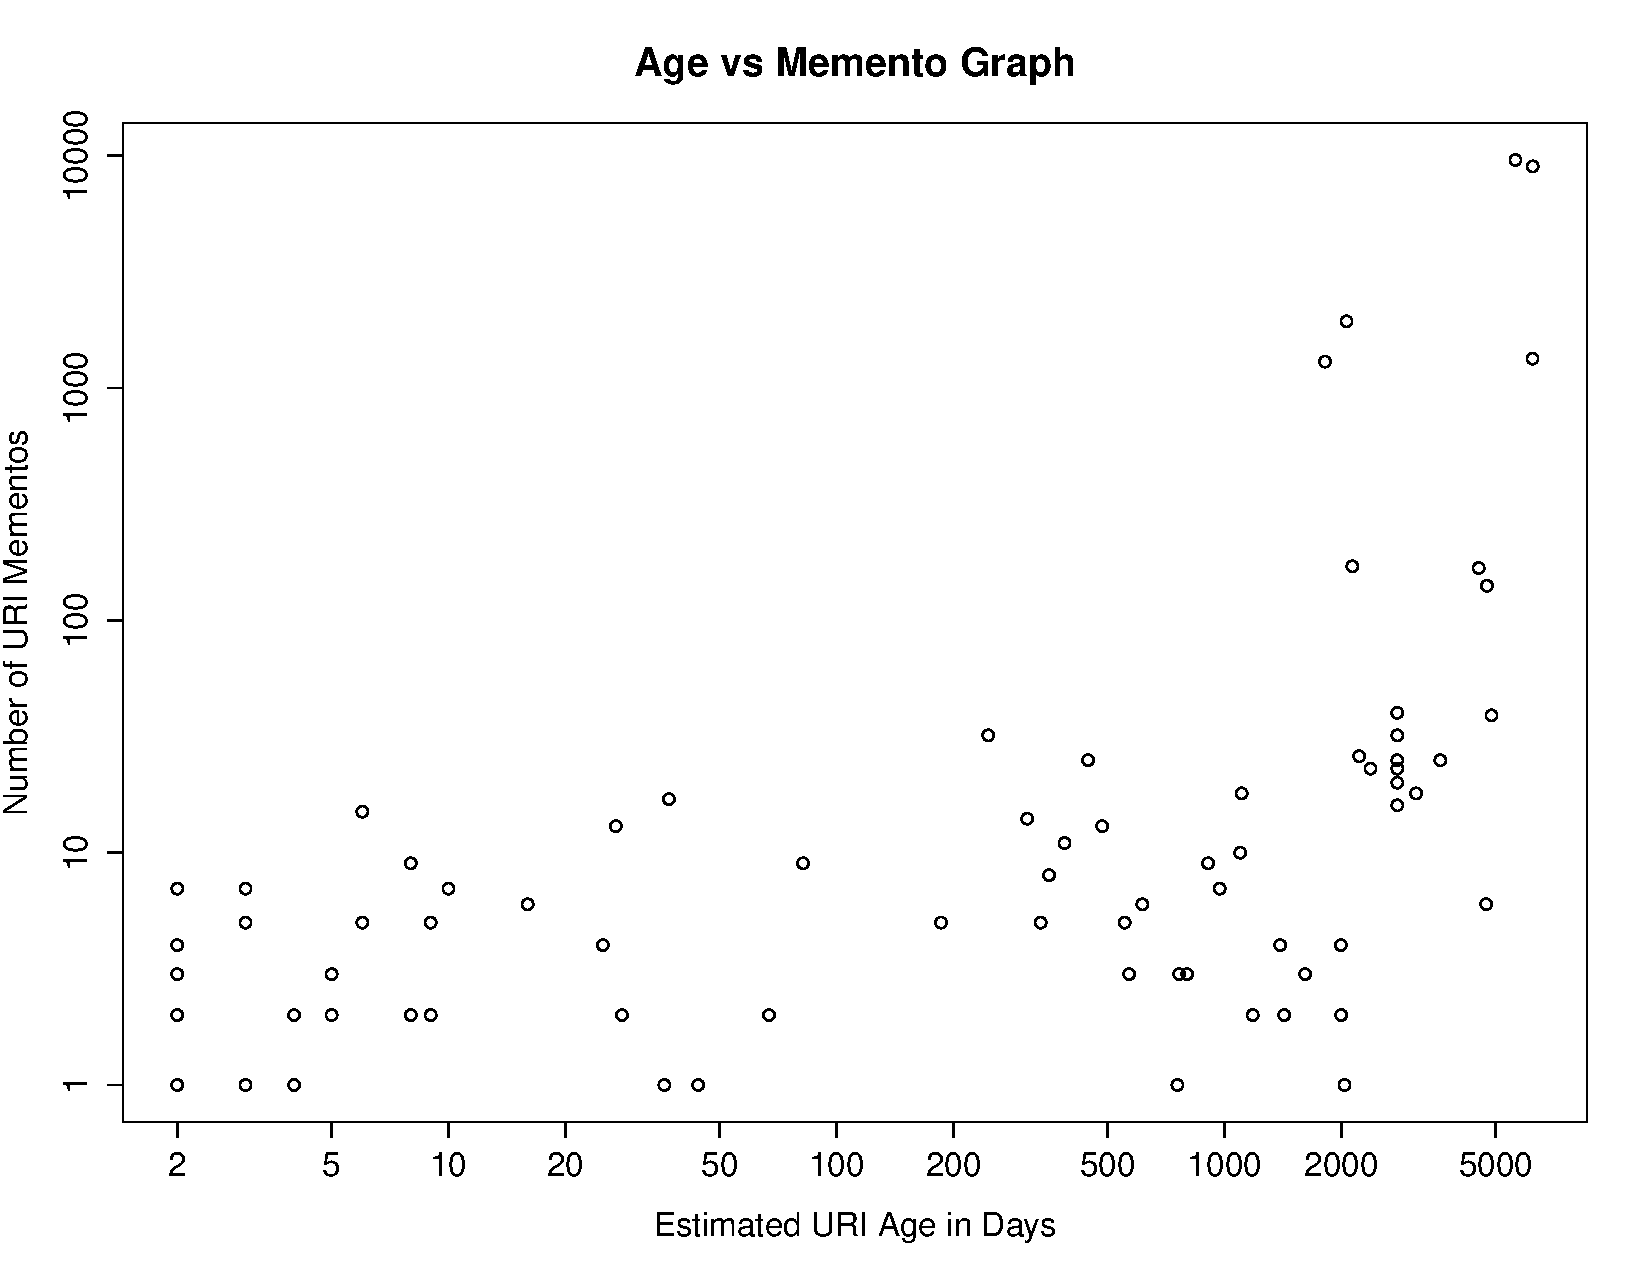
\includegraphics[scale=.5]{images/original-age-memento.pdf}
\caption*{\scriptsize The x-axis and y-axis are in a log scale.  The data used to plot this graph is contained in Table \ref{tab:table2}. Number of plotting points do not correspond to number of data set in Table \ref{tab:table2} due to tuple value repetition with different URIs. It is difficult to appreciate repeating plots with darker plotting points on this graph. Then, it is a need to capture plot point repetition: Figure \ref{fig:5}.}
\end{figure}
From the graph above we can notice a relationship between an URI's age and its Mementos count. In general, the younger the URI the less count of mementos it has, and vice versa. Figure \ref{fig:5} captures much better this inference, since the plot density is more representative of the collected data. 

\newpage
\begin{figure}[!h]
\caption{Age-Memento Graph with Various Plot Size}\label{fig:5}
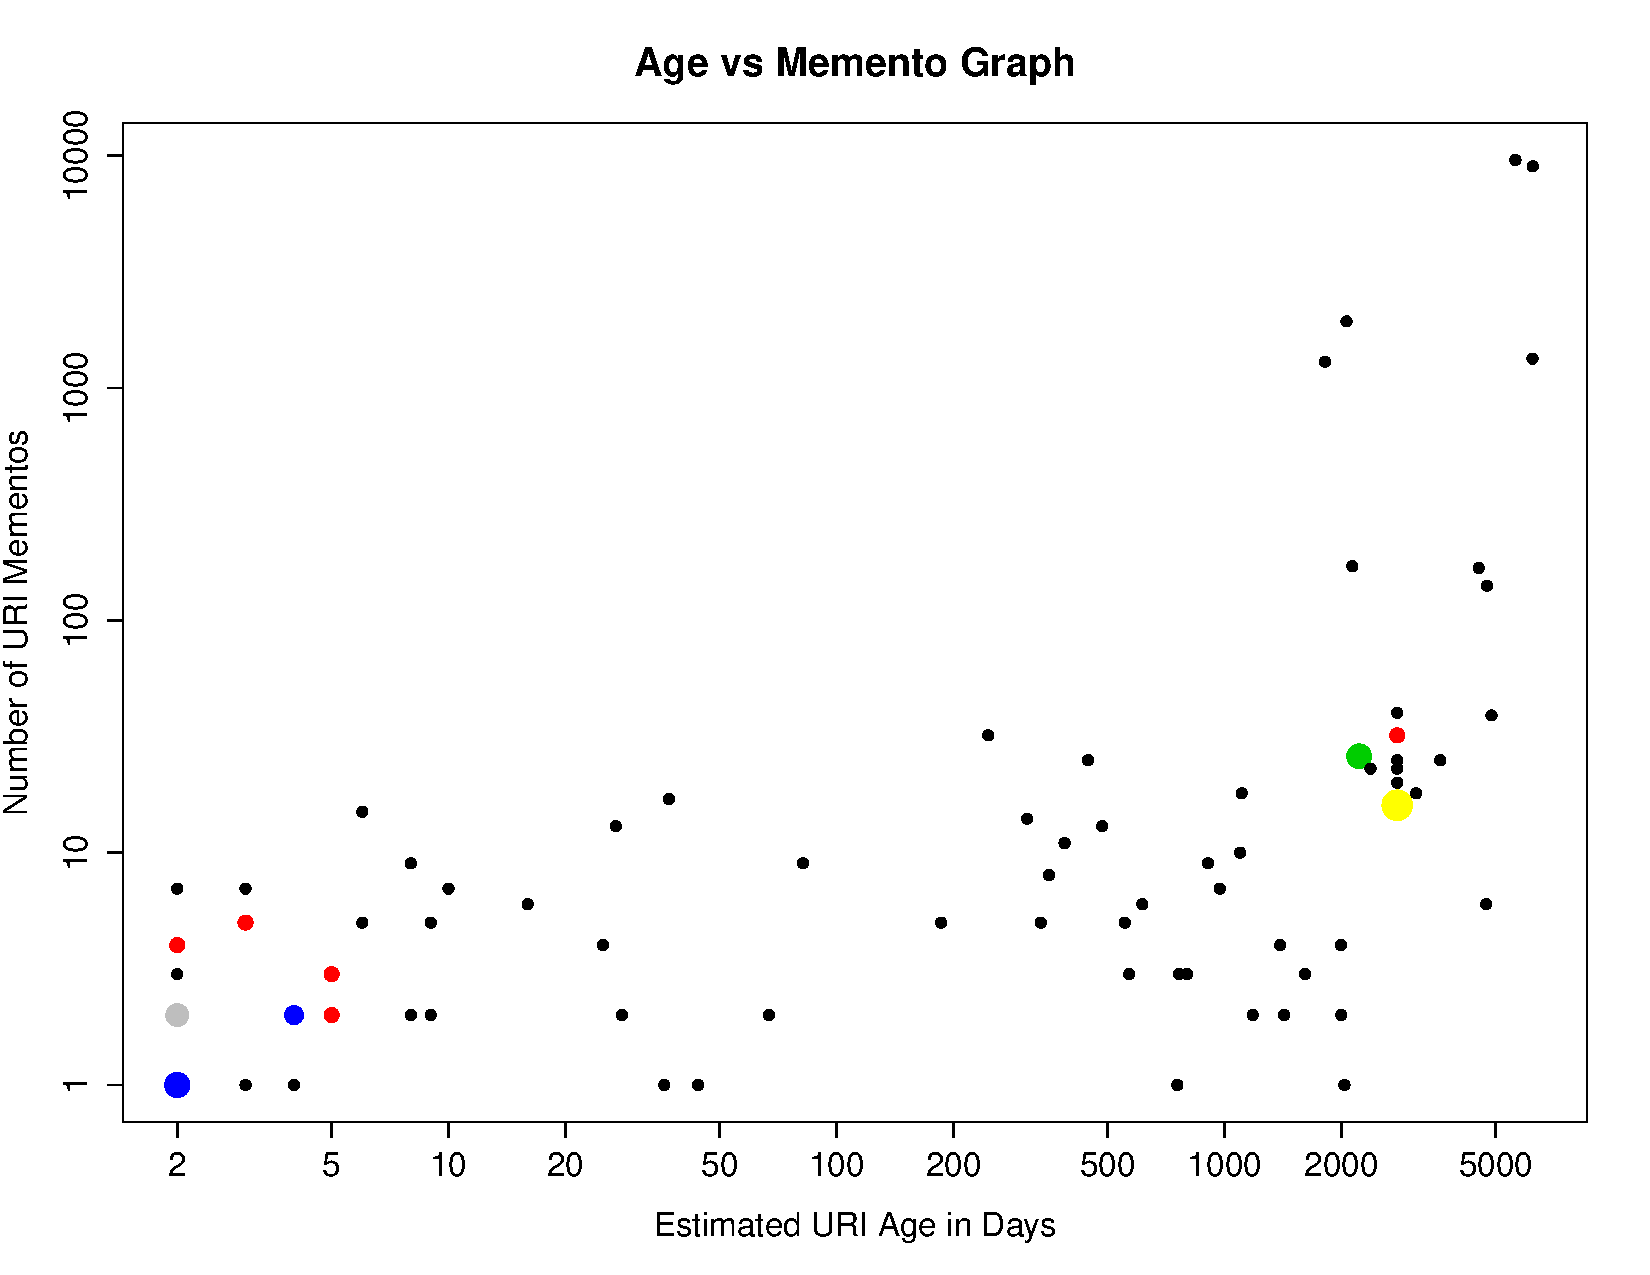
\includegraphics[scale=.5]{images/update-age-memento.pdf}
\caption*{\scriptsize The x-axis and y-axis are in a log scale.  The data used to plot this graph is contained in Table \ref{tab:table3}. The plot point size corresponds to column labeled \textit{Freq} from the same table utilizing the formula: $log\ Freq/2 + 1$. The larger the plot point size, the greater the number of occurrences for any particular data set.}
\end{figure}
%
The analysis of Figure \ref{fig:5} is similar to Figure \ref{fig:4}. In general, the younger the URI the less count of mementos it has, and vice versa. However, the plotting is more representative of its data. For example, we can appreciate that a great deal of pages 2 days old have 1 memento. This information is not capture on Figure \ref{fig:4}.
%
\subsection{3.3 Solution Part-2}
Not all URIs will have Mementos, and not all URIs will have an estimated creation date. \textit{\textbf{AgeURI.py}} calculated this information:\\

Out of 1000 URIs 382 or 38.20\% have no estimated creation date.\\
Out of 1000 URIs 860 or 86.00\% have no mementos.\\

Additionally, the number of URIs with an estimated creation date and a memento is 140 or 14.00\%.
\end{homeworkProblem}

%----------------------------------------------------------------------------------------
%	Tables
%----------------------------------------------------------------------------------------
\import{./}{tables.tex}

%----------------------------------------------------------------------------------------
%	Bibliography
%----------------------------------------------------------------------------------------
\newpage
\begin{thebibliography}{9}
\bibitem{Lutz} 
Lutz, Mark (2013). List and Dictionaries. \textit{Learning Python} (5th ed.). (pp. 262-263). Sebastopol, CA: O'Reilly Media.
%\bibitem{Graph structure in the web}
%Graph structure in the web. (n.d.) Retrieved January 23, 2016, from \url{http://%http://www9.org/w9cdrom/160/160.html}
\end{thebibliography}
\end{document}